\section{Implementation}
\label{sec:impl}

We chose to implement and run our policies on a Samsung Galaxy Nexus running Android 4.2 Jelly Bean. The Galaxy Nexus runs on AT\&T's 3G HSPA+ network. It was released late 2011 and is widely used today.

Originally, we aimed to modify Android's source code in order to implement our policies. This would have given us a great degree of control over Android's WiFi decision making policies. However, Android's source is not extensively documented and poorly understood outside of its group of core developers as Google \cite{Yaghmour:2013} Therefore, our best option became implementing our policies as an Android application running on top of the OS's pre-existing WiFi management policies.

As we will discuss, this created sub-optimal conditions for the policies. Because the application ran on top of Android's WiFi management code, we faced several limitations. In addition to only being able to access the WiFi state via Android's APIs our application had to compete with Android's internal WiFi management. We will make clear how this affected our implementation, and how we expected it to affect our evaluation.

The application itself allows users to select one of three policies: internet access testing (Bouncer), predictive WiFi abandonment (AbandonShip), and unmodified Android WiFi policies. When the policy was selected, an Android broadcast receiver was registered. Broadcast receivers are Android objects which subscribe to messages published by the Android system. Our broadcast receivers subscribed to changes in the device's network connection (i.e. a WiFi connection was established). When connected to WiFi, these receivers would start the appropriate policy.

% [This is being left out as redundant]
% In order to evaluate how each of these policies affected Internet connectivity, the application sent UDP packets approximately every 100 milliseconds to a server on the Internet. This allowed us to gather data about when WiFi connections were usable and providing reliable internet connectivity.

\subsection{Internet Access Testing - Bouncer}
Our implementation of internet access testing, Bouncer, was written as a thread spawned by the broadcast receiver to perform the necessary tests. This was choosen over running the policy as a service, an Android construct used for doing long-running background work. Since the thread has to be active only as long as network testing occurs (in our case, about 3 seconds), we felt that running it as a service would be wasteful.

The thread attempted to ping a well known web site (umich.edu). If the server responded with an HTTP OK response code (200), the thread would sleep for 3 seconds before running again. This was repeated twice. If a test failed, the connection was abandoned, and the device was forced to use its cellular data connection.

Optimally, we would have tested new networks as the device came into contact with them, before tearing down the cell network connection, joining one if and only if it passes all testing. However, because Bouncer was implemented as an application, not at the operating system level, we could not prevent the device from joining WiFi networks.

Our solution was to, as soon as the device joined a new WiFi network, test its connectivity. If all tests were passed, the thread ended and the WiFi connection was left untouched. However, if a network failed any of the tests, we disconnected from the network, forcing it to use the cellular data connection.

Were the policy optimally implemented, we would have expected no downtime, assuming a usable cellular data connection. All WiFi Internet access testing would occur without disconnecting from cellular data, allowing applications to continue to use the cellular data connection. The switch would then be made if and only if all tests were passed by the WiFi network.

However, because of the limitations imposed upon us, we had to force the device to disconnect from unsuitable WiFi networks after Android had decided to join them. This, we expected, would lead to downtime while the device was connected to an unsuitable network and as the device moved back from WiFi to cellular data. Again, were we to have greater access to Android's internals, we would be able to prevent utilization of the WiFi connection entirely until it had passed our tests.

\subsection{Predictive WiFi Abandonment - AbandonShip}
Our implementation of predictive WiFi abandonment, AbandonShip, was written as an Android service spawned by the broadcast receiver. When a WiFi connection was established, a service was started in the background. That service would monitor the WiFi network's signal strength over time.

Given a certain strength threshold (-80 RSSI units) and timeout (6.9 seconds), the service monitored signal strength in order to determine whether the signal had degraded below the strength threshold for a time equal to or greater than the timeout. We estimated these experimental values from data, such as that presented in figure 1, demonstrating WiFi signal strength as recorded by Android. 

This data was kept in a single variable: the count of consecutive signal strength readings below the strength threshold. Whenever the signal strength exceeded the strength threshold, the count was reset to 0.

\begin{figure}
	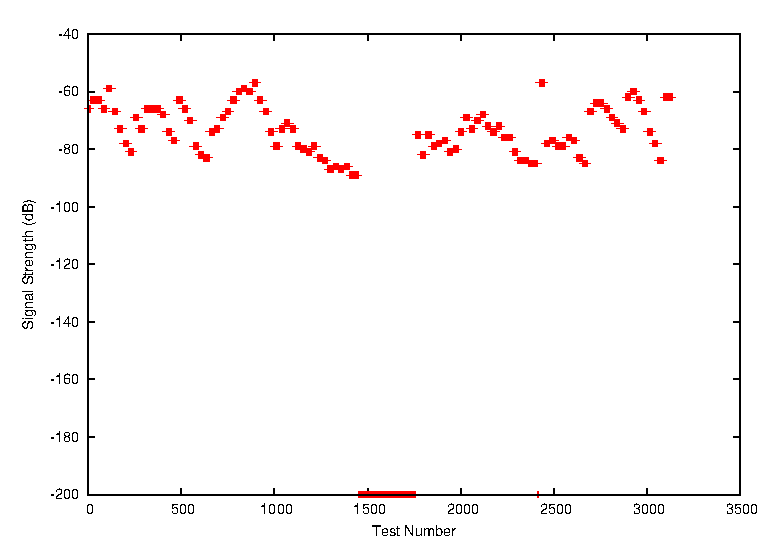
\includegraphics[width=0.5\textwidth]{sigStrength}
	\caption{TODO}
\end{figure}

Because signal strength was sampled approximately every 100 milliseconds, the duration of signal strength below the strength threshold in seconds could be calculated by multiplying the sub-strength reading count by 0.1. For example, 42 consecutive packets below the strength threshold corresponded to $ 42 \cdot 0.1 = 4.2 $ seconds.

When the calculated time exceeded the timeout, the system determineed that the connection was becoming weaker, and would likely degrade past the point of usability. It then disconnected from the WiFi network, forcing the device to utilize its cellular data connection.

Like Bouncer, this implementation would have benefited from a lower-level implementation. However, the hindrance on AbandonShip is not as great. The only problem is that Android does not know to expect the disconnection from WiFi. The sudden disconnection ``surprises" it, and, as we will see in the evaluation, causes some downtime as Android switches to the cellular data network. Had we access to lower level networking, we could start re-establishing the cellular data connection part way through the time out, so that we could move seemlessly to it when the WiFi was deemed unusable
.